% !TEX program = xelatex
\documentclass[11pt,a4paper]{article}
\usepackage{fontspec}
\setmainfont{TeX Gyre Termes}
\usepackage[a4paper,margin=23mm,headheight=16pt]{geometry}
\usepackage{amsmath,amssymb,booktabs,graphicx,xcolor,fancyhdr,lastpage,hyperref,enumitem,caption}
\definecolor{CoursePurple}{HTML}{5C2267}
\hypersetup{colorlinks=true,linkcolor=CoursePurple,urlcolor=CoursePurple,pdftitle={DDA5001 Homework 2},pdfauthor={Kunyuan Zhong}}
\pagestyle{fancy}\fancyhf{}
\fancyhead[L]{\small DDA5001 Machine Learning}\fancyhead[R]{\small Homework 2}
\fancyfoot[R]{\small\thepage/\pageref*{LastPage}}
\setlength{\parindent}{0pt}\setlength{\parskip}{5pt}\setlength{\emergencystretch}{3em}
\setlist[enumerate]{leftmargin=1.6em,itemsep=3pt,topsep=3pt}
\captionsetup{font=small,labelfont=bf,skip=4pt}
\newcommand{\R}{\mathbb R}
\newcommand{\Ein}{E_{\mathrm{in}}}
\newcommand{\Eout}{E_{\mathrm{out}}}
\newcommand{\Th}{\Theta}
\newcommand{\softmax}{\operatorname{softmax}}
\newcommand{\method}{\texttt}
\begin{document}
\begin{center}{\Large\bfseries\color{CoursePurple}DDA5001 Homework 2}\\[4pt]
The Chinese University of Hong Kong, Shenzhen\\[2pt]
\small Kunyuan Zhong \quad Student ID: 226040255
\end{center}
\noindent\rule{\linewidth}{0.8pt}

\section*{Problem 1: Concepts and fundamental knowledge}
\textbf{(a) VC dimension.} The VC dimension is $d+1$ for affine binary linear classifiers in $\R^d$, where the appended constant feature supplies the intercept. The $d+1$ affinely independent vertices of a simplex can be shattered. The standard upper bound for affine halfspaces rules out shattering $d+2$ points. The feature count $d$ here excludes the constant coordinate.

\textbf{(b) Test error versus out-of-sample error.} For a fixed learned classifier $h$, its out-of-sample classification error is the population probability
\[
\Eout(h)=\mathbb P_{(x,y)\sim P}\{h(x)\ne y\}.
\]
The test error is the observed fraction of mistakes on a finite held-out test sample:
\[E_{\mathrm{test}}(h)=\frac1m\sum_{j=1}^m\mathbf 1\{h(x_j)\ne y_j\}.\]
It varies with the test sample and estimates the population error; with i.i.d. test examples independent of learning, its expectation conditional on the fixed $h$ equals $\Eout(h)$. The two quantities need not be numerically equal.

\textbf{(c) Gradient descent: statement 2 is false.}
\begin{enumerate}[label=\arabic*)]
\item True. Convexity gives $L(u)\ge L(\theta)+\nabla L(\theta)^\top(u-\theta)$. A zero gradient therefore implies $L(u)\ge L(\theta)$ for every $u$.
\item False. For $L(\theta)=\theta^2$, one update is $\theta^+=(1-2\mu)\theta$. If $\mu>1$ and $\theta\ne0$, then $L(\theta^+)>L(\theta)$. Convexity alone cannot control an arbitrarily large step.
\item True. For $g=\nabla L(\theta)\ne0$, differentiability gives $L(\theta-\alpha g)=L(\theta)-\alpha\|g\|^2+o(\alpha)$. This decreases for sufficiently small positive $\alpha$.
\item True. The iterate displacement is $\mu\|\nabla L(\theta)\|$ and can be tiny because $\mu$ is tiny. For the same quadratic, an arbitrarily small learning rate can give a tiny displacement far from the minimizer $0$.
\end{enumerate}

\textbf{(d) Softmax: statement 3 is false.}
\begin{enumerate}[label=\arabic*)]
\item True. Exponentiation preserves ordering and all classes share the same positive denominator; the sets of maximizers, including ties, coincide.
\item True. Adding $c$ multiplies numerator and denominator by $e^c$, which cancels.
\item False. Scaling scores changes their differences and typically changes the probabilities. For scores $(0,1)$, the second probability is $e/(1+e)$; after scaling by $2$ it is $e^2/(1+e^2)$. A positive scale preserves the predicted class, but not these probabilities.
\item True. If the true class is $y$, one-hot cross-entropy reduces to $-\log q_y$.
\end{enumerate}

\clearpage
\section*{Problem 2(a): Analytic mean cross-entropy gradient}
For one sample, use $z=\Th^\top x$, $q=\softmax(z)$ and one-hot $p$ with $\sum_jp_j=1$. Softmax probabilities are strictly positive in exact arithmetic.

\textbf{Step 1: differentiate cross-entropy.}
\[
H(p,q)=-\sum_{j=1}^K p_j\log q_j,
\qquad \boxed{\frac{\partial H}{\partial q_j}=-\frac{p_j}{q_j}.}
\]

\textbf{Step 2: differentiate with respect to the logits.} Separating $j=k$ from the other terms in the chain rule gives
\begin{align*}
\frac{\partial H}{\partial z_k}
&=-\frac{p_k}{q_k}q_k(1-q_k)
 +\sum_{j\ne k}\left(-\frac{p_j}{q_j}\right)(-q_jq_k)\\
&=-p_k+p_kq_k+q_k\sum_{j\ne k}p_j
 =-p_k+q_k\sum_jp_j=q_k-p_k.
\end{align*}
Hence $\boxed{\nabla_z H=q-p\in\R^K}$.

\textbf{Step 3: differentiate the parameter columns.} Since $z_k=\theta_k^\top x$ and only column $\theta_k$ affects $z_k$,
\[
\nabla_{\theta_k}H=x(q_k-p_k),\qquad
\boxed{\nabla_{\Th}H=x(q-p)^\top\in\R^{d\times K}.}
\]
The outer product has features as rows and classes as columns.

\textbf{Step 4: average over samples.}
\[
\boxed{\nabla_{\Th}L(\Th)=\frac1n\sum_{i=1}^n x_i(q_i-\mathbf 1_i)^\top
       =\frac1n X^\top(P-Y).}
\]
Here $X\in\R^{n\times d}$ has sample rows; $P=\softmax(X\Th)$ and $Y\in\R^{n\times K}$ have probability and one-hot rows. The factor $1/n$ corresponds to the mean loss, not a sum loss.

\section*{Problem 2(b): Implementation and fixed experiment}
The six functions are in \method{p2/algorithms.py}. Softmax subtracts each row maximum $m$ before exponentiation. Since $e^{z_j-m}/\sum_\ell e^{z_\ell-m}=e^{z_j}/\sum_\ell e^{z_\ell}$, this is the same distribution. The loss uses
\[
\log q_j=(z_j-m)-\log\sum_\ell e^{z_\ell-m},
\]
then averages $-\sum_jp_j\log q_j$. Thus it avoids $\log(0)$ after probability underflow, without clipping. Training uses the analytic matrix gradient, no autodiff, ready-made optimizer or classifier. All updates return new arrays.

For updates $k=1,\ldots,1000$, with $\Th_0=\Th_1=0$, $\mu=0.05$ and $\beta=0.90$,
\begin{align*}
\text{GD:}\quad&\Th_{k+1}=\Th_k-\mu\nabla L(\Th_k),\\
\text{Momentum:}\quad&\Th_{k+1}=\Th_k-\mu\nabla L(\Th_k)+\beta(\Th_k-\Th_{k-1}),\\
\text{Nesterov:}\quad&W_k=\Th_k+\frac{k-1}{k+2}(\Th_k-\Th_{k-1}),\quad
\Th_{k+1}=W_k-\mu\nabla L(W_k).
\end{align*}
Each update uses exactly one full-training-set gradient. The original framework fixes seed 666, stratified 80/20 splitting after exact deduplication, training-only standardization and an appended constant feature, without regularization. No test observations enter a gradient. Parameters have shapes $65\times10$ (Digits) and $17\times7$ (Dry Bean). The recorded iteration is the number of completed updates.

\clearpage
\section*{Problem 2(b): Numerical verification before training}
\textbf{Gradient check.} The supplied four-sample input, labels and parameter matrix were used:
\[
X=\begin{pmatrix}1&-1&1\\2&0.5&1\\-1&2&1\\0.5&0.2&1\end{pmatrix},\quad
Y=\begin{pmatrix}1&0&0\\0&1&0\\0&0&1\\0&1&0\end{pmatrix},\quad
\Th=\begin{pmatrix}0.1&-0.2&0.05\\0.3&-0.1&0.2\\0.02&0.1&-0.1\end{pmatrix}.
\]
For each entry, the central difference is
\[
(G_{\rm FD})_{ab}=\frac{L(\Th+10^{-6}E_{ab})-L(\Th-10^{-6}E_{ab})}{2\times10^{-6}}.
\]
The computed analytic and numerical matrices are, respectively,
\[G_{\rm analytic}=\begin{pmatrix}-0.0050469778 & -0.4493466297 & 0.4543936075\\0.4507050638 & -0.0919780778 & -0.3587269860\\0.1365728698 & -0.2029764344 & 0.0664035646\end{pmatrix}\]
\[G_{\rm FD}=\begin{pmatrix}-0.0050469777 & -0.4493466297 & 0.4543936075\\0.4507050638 & -0.0919780777 & -0.3587269860\\0.1365728699 & -0.2029764343 & 0.0664035645\end{pmatrix}\]
The maximum entrywise absolute difference, before rounding the displayed matrices, is $1.174011\times10^{-10}$. This is below $10^{-8}$ and supports agreement with the mean-loss gradient in part (a).

\textbf{One accelerated update.} Set $\Th_{\rm previous}=\Th-0.02$ entrywise, $\mu=0.05$, $\beta=0.90$, $k=3$ and $G(A)=2A$. Momentum evaluates $G$ at the current matrix $\Th$ displayed above and returns
\[\Th^+_{\rm Momentum}=\begin{pmatrix}0.1080 & -0.1620 & 0.0630\\0.2880 & -0.0720 & 0.1980\\0.0360 & 0.1080 & -0.0720\end{pmatrix}.\]
Nesterov uses $(k-1)/(k+2)=2/5$, so its recorded gradient point is\[W=\Th+0.008=\begin{pmatrix}0.1080 & -0.1920 & 0.0580\\0.3080 & -0.0920 & 0.2080\\0.0280 & 0.1080 & -0.0920\end{pmatrix},\]
and its computed updated parameter is\[\Th^+_{\rm Nesterov}=\begin{pmatrix}0.0972 & -0.1728 & 0.0522\\0.2772 & -0.0828 & 0.1872\\0.0252 & 0.0972 & -0.0828\end{pmatrix}.\]
These match the separate formula calculations $0.9\Th+0.018$ and $0.9(\Th+0.008)$. Both gradient points match their expectations exactly in the check; both update discrepancies are $2.776\times10^{-17}$ (rounding), with one gradient call each. Momentum uses the current point and adds the previous displacement afterward. Nesterov extrapolates first and evaluates the gradient at that extrapolated point.

\textbf{Additional checks.} All seven supplied P2 tests passed before the full runs. The loss on logits $(1000,-1000)$ with the second class true is $2000$ (expected $2000$); zero logits with three classes give $\log3=1.0986122887$. Stability, shift invariance, first-update equality and unchanged inputs also passed. The included \method{p2/verify.py} prints these numerical checks without downloading a dataset.


\clearpage
\section*{Problem 2(b): Digits learning curves}
\begin{center}
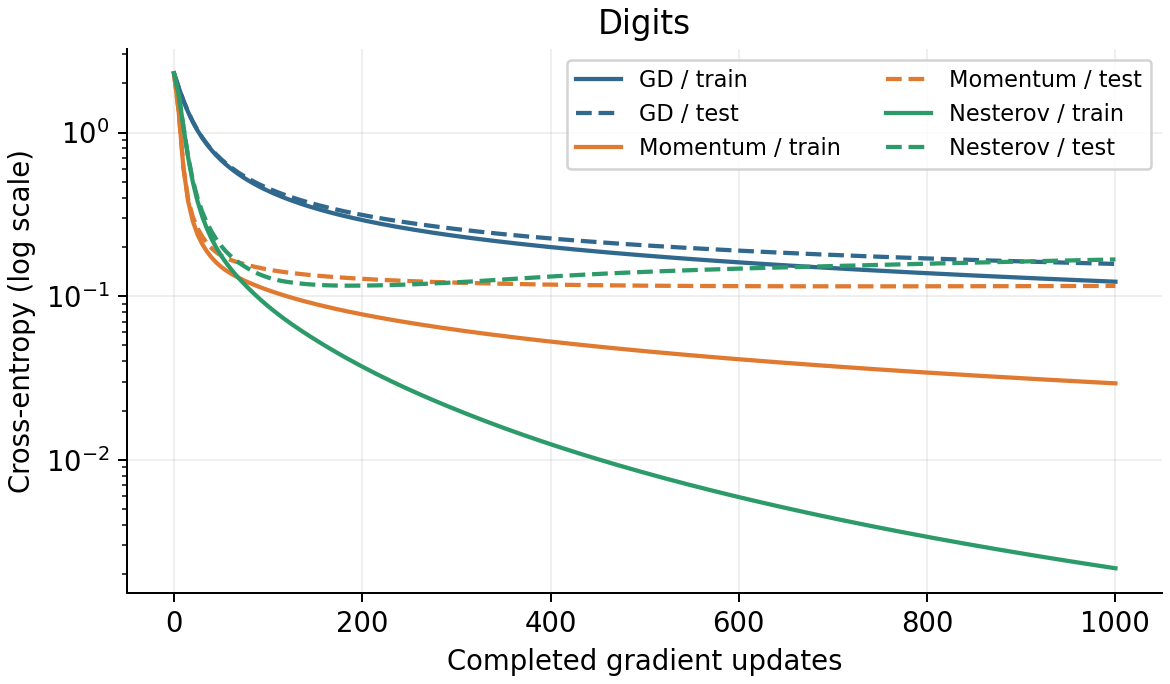
\includegraphics[width=.96\linewidth]{../results/run-20261027/p2/digits_loss.png}
\captionof{figure}{Digits mean cross-entropy on a logarithmic vertical axis. Each of the three methods has a training curve and a test curve.}\label{fig:digits-loss}
\end{center}
\begin{center}
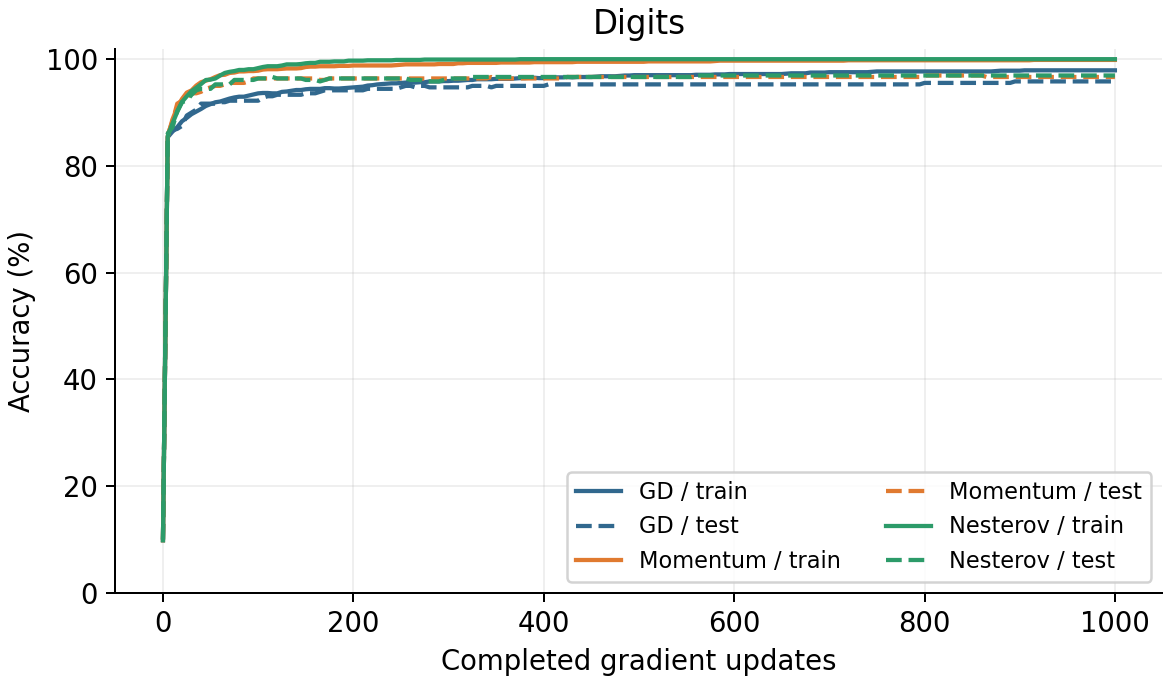
\includegraphics[width=.96\linewidth]{../results/run-20261027/p2/digits_accuracy.png}
\captionof{figure}{Digits accuracy. Solid lines are training and dashed lines are test. Values are recorded after updates $0,5,\ldots,1000$.}\label{fig:digits-accuracy}
\end{center}

\clearpage
\section*{Problem 2(b): Dry Bean learning curves}
\begin{center}
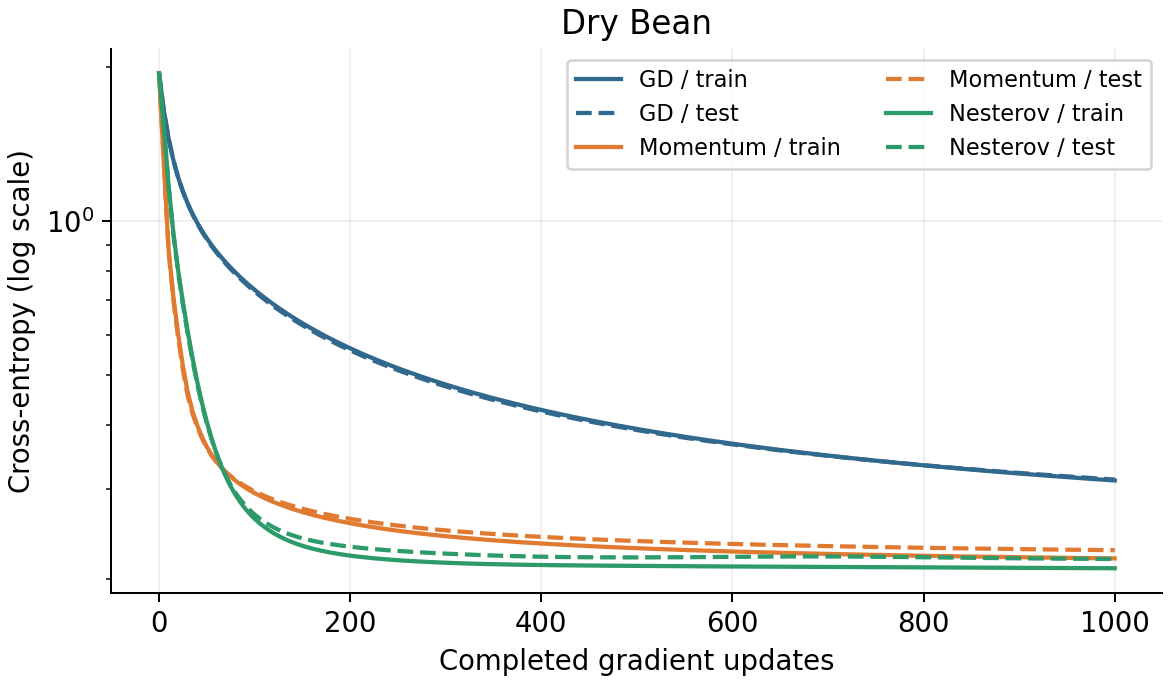
\includegraphics[width=.96\linewidth]{../results/run-20261027/p2/dry_bean_loss.png}
\captionof{figure}{Dry Bean mean cross-entropy on a logarithmic vertical axis, using the same fixed methods and settings as Digits.}\label{fig:bean-loss}
\end{center}
\begin{center}
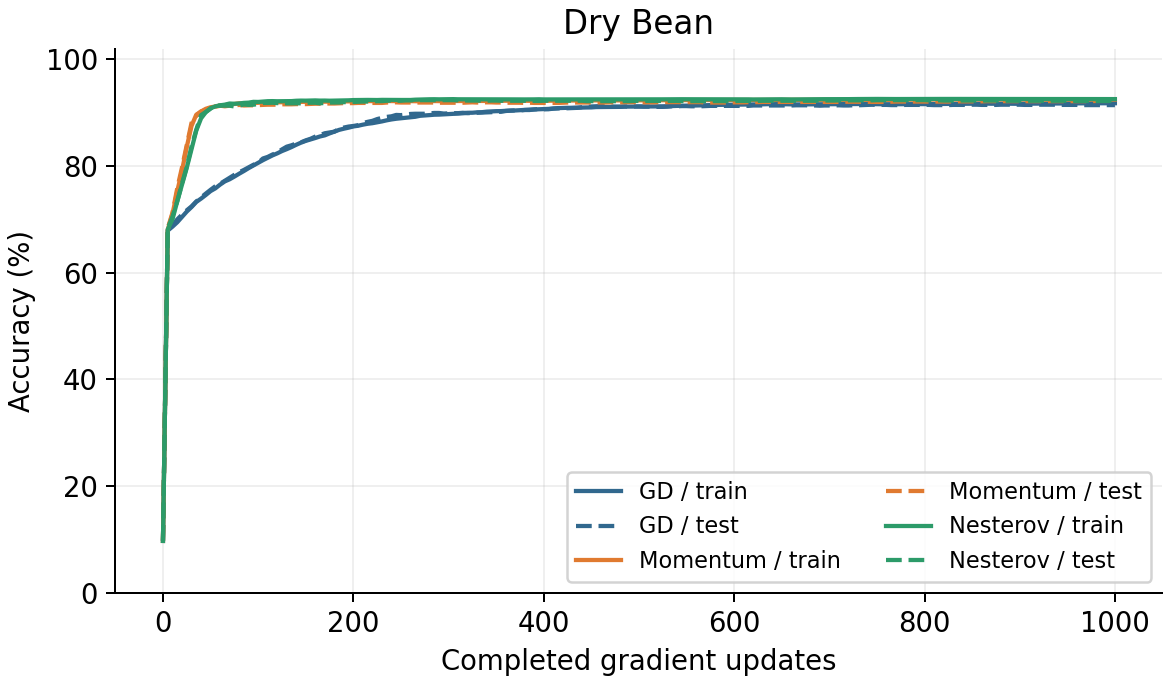
\includegraphics[width=.96\linewidth]{../results/run-20261027/p2/dry_bean_accuracy.png}
\captionof{figure}{Dry Bean accuracy. Each figure contains all six training/test curves; the held-out set is used only for evaluation.}\label{fig:bean-accuracy}
\end{center}

\clearpage
\section*{Problem 2(b): Results and interpretation}
\textbf{Dataset sizes.} Digits has 1437 training and 360 test examples, with no exact duplicates removed. Dry Bean has 10834 training and 2709 test examples after removing 68 duplicates (13543 remaining). These sizes and the train/test hashes were recorded by the unmodified framework.

\begin{table}[htbp]\centering\small
\caption{Metrics after exactly 1000 updates. CE denotes mean cross-entropy; accuracy is a percentage.}\label{tab:p2}
\begin{tabular}{@{}llrrrr@{}}\toprule
Dataset & Method & Train CE & Test CE & Train acc. & Test acc.\\\midrule
Digits & GD & 0.122606 & 0.157478 & 97.912\% & 95.833\%\\
Digits & Momentum & 0.029333 & 0.115559 & 99.861\% & 96.667\%\\
Digits & Nesterov & 0.002176 & 0.167670 & 100.000\% & 96.944\%\\
Dry Bean & GD & 0.311315 & 0.312644 & 91.748\% & 91.399\%\\
Dry Bean & Momentum & 0.219241 & 0.227494 & 92.431\% & 92.174\%\\
Dry Bean & Nesterov & 0.209742 & 0.218661 & 92.524\% & 92.174\%\\
\bottomrule\end{tabular}\end{table}

\textbf{(i) Which method reduces training loss faster?} In these runs, Nesterov eventually reduces training loss fastest, Momentum is next, and GD is slowest on both datasets. At update 100, the training CE values for GD/Momentum/Nesterov are $0.439801/0.108877/0.086856$ on Digits and $0.734252/0.294142/0.262083$ on Dry Bean. The final training losses have the same ordering. This is a comparison at equal gradient-update budgets, rather than a claim that one curve is lower at every early iteration.

\textbf{(ii) Which method has the best final test metrics?} On Digits, Momentum has the lowest test CE ($0.115559$), while Nesterov has the highest test accuracy ($96.944\%$). Nesterov has the lowest training CE but a higher test CE ($0.167670$) than both other methods. Accuracy measures only the winning class; CE also penalizes confident incorrect predictions, so their rankings can differ. On Dry Bean, Nesterov has the lowest test CE ($0.218661$), and Nesterov and Momentum tie for the highest test accuracy ($92.174\%$, exactly the same accuracy before rounding). Thus the lowest-training-loss method is best on test CE for Dry Bean, but not for Digits.

\textbf{(iii) Is there evidence of overfitting?} On Digits, Nesterov's smallest recorded test CE is $0.115969$ at update 185; its training CE there is $0.041322$. By update 1000, training CE falls to $0.002176$ while test CE rises to $0.167670$. Momentum has a weaker instance: after its test CE minimum of $0.114851$ at update 730, training CE falls from $0.036272$ to $0.029333$, while test CE increases to $0.115559$. The loss curves therefore show a divergence between continued fitting of training examples and held-out log-loss performance. In the last 100 updates, test CE increases by $0.004749$ for Nesterov and $0.000392$ for Momentum while each training CE decreases.

For Dry Bean, no sustained late training/test loss divergence is observed. All three methods attain their lowest recorded test CE at update 1000, and both losses decrease over the last 100 updates. This does not prove that the models cannot overfit with a different training duration or setting. Test minima above are descriptive observations only; the prescribed final update remains 1000 and no stopping rule or hyperparameter was selected using the test set.


\clearpage
\section*{Problem 2(b): AI collaboration case}
\textbf{Decision being checked.} This case concerns whether the Nesterov implementation evaluates its gradient at the prescribed lookahead point. Implementation and checks preceded this student verification discussion. The actual student--Codex messages below are translated from Chinese; the originals are retained in this chat and locally. Tool: Codex; no more specific model identifier was displayed.

\textbf{Student's initial concern and actual prompt.}
\begin{quote}\small
``Why does Nesterov evaluate the gradient at the lookahead point, and can the existing $k=3$ check distinguish an incorrect evaluation point?''
\end{quote}

\textbf{Relevant response excerpt (English translation).}
\begin{quote}\small
``Nesterov first uses the previous displacement to form a lookahead point $W$, then corrects it using the gradient at $W$; this is the update formula specified in this assignment. Evaluating the gradient at the current parameter $\Theta$ instead would give a different update.''
\end{quote}
Codex then explained the existing prescribed check: $\Theta-\Theta_{\mathrm{previous}}=0.02$ entrywise, $k=3$, $\mu=0.05$, and $G(A)=2A$. Thus $W=\Theta+(2/5)(0.02)=\Theta+0.008$ and
\[
\underbrace{W-0.05(2W)}_{\text{correct}}=0.9\Theta+0.0072,\qquad
\underbrace{W-0.05(2\Theta)}_{\text{wrong gradient point}}=0.9\Theta+0.008.
\]
The incorrect result differs by $0.0008$ in every entry. Codex reported that the implemented function recorded the point $W$ and that its update differed from the correct formula by only $2.78\times10^{-17}$. It also explained why a first-step-only check would miss the distinction: the first extrapolation coefficient is zero.

\textbf{Numerical evidence brought back and focused follow-up.} After this response, the student asked (English translation):
\begin{quote}\small
``The result shows a one-step error of only $2.78\times10^{-17}$, whereas an incorrect evaluation point would differ by $0.0008$: is this enough to retain the current code, and what else needs checking?''
\end{quote}
This follow-up was selected and submitted by the student from a suggested question in the chat. The numerical evidence was calculated by the verification script, rather than being claimed as a manual student calculation.

\textbf{Relevant follow-up response and final action.} Codex answered that these values support retaining the gradient location, while one check alone does not establish correctness of the whole program. It identified the analytic gradient, update count, one gradient call per update, nonmutation and exclusion of test data from training as further checks. It then reported that all 15 supplied tests passed and a separate Verifier checked other iterations and data leakage and reproduced both complete experiments in a fresh environment, with identical results. Codex's actual concluding decision was (English translation):
\begin{quote}\small
``Therefore I will retain the current code without modification, and include your numerical follow-up and this decision in the AI case.''
\end{quote}

\textbf{Final decision (AI-assisted wording).} When asked to state the final decision, the student replied, ``Please write it for me'' (English translation). At that explicit request, Codex drafted: \emph{Retain the current implementation because the $k=3$ check records the gradient at the prescribed point, its update discrepancy is at floating-point rounding scale, and the other tests and independent full reproductions passed.} The code was retained without modification. This is disclosed as assisted drafting, not an independently worded student endorsement. The matrices and unrounded discrepancies are on page~3 and are regenerated by \method{p2/verify.py}. The gradient discrepancy is $1.174011\times10^{-10}$ (tolerance $10^{-8}$); the update tolerance is $10^{-14}$. No bug, student calculation or extra exchange was invented.


\clearpage
\section*{Problem 3(a): Least-squares Legendre fits}
For degree $K$, define
\[
A_K=\begin{pmatrix}
L_0(x_1)&L_1(x_1)&\cdots&L_K(x_1)\\
L_0(x_2)&L_1(x_2)&\cdots&L_K(x_2)\\
\vdots&\vdots&&\vdots\\
L_0(x_n)&L_1(x_n)&\cdots&L_K(x_n)
\end{pmatrix},\quad
w^{(K)}=\begin{pmatrix}w_0\\w_1\\\vdots\\w_K\end{pmatrix},\quad
y=\begin{pmatrix}y_1\\y_2\\\vdots\\y_n\end{pmatrix}.
\]
Then $A_K\in\R^{n\times(K+1)}$, $w^{(K)}\in\R^{K+1}$ and $y\in\R^n$. In particular, $A_2$ has rows $(1,x_i,(3x_i^2-1)/2)$ and $A_{10}$ has rows $(L_0(x_i),\ldots,L_{10}(x_i))$.

A nonzero linear combination of these basis polynomials has degree at most $K$, so it cannot vanish at $K+1$ distinct inputs. Thus the assumed $n\ge K+1$ distinct samples imply full column rank. Differentiating the mean squared training error gives
\[
\nabla_w\left(\frac1n\|A_Kw-y\|_2^2\right)=\frac2nA_K^\top(A_Kw-y)=0.
\]
Since $A_K^\top A_K$ is positive definite, the unique minimizer is
\[
\boxed{\widehat w^{(2)}=(A_2^\top A_2)^{-1}A_2^\top y,\qquad
\widehat w^{(10)}=(A_{10}^\top A_{10})^{-1}A_{10}^\top y.}
\]
These inverses describe the mathematical solution. The implementation uses \method{numpy.linalg.lstsq(A, y, rcond=None)} to solve it numerically without forming the normal-equation inverse. For batched labels, each column is fitted independently using the same $A_K$. No oracle target coefficients enter fitting.

\section*{Problem 3(b): Analytic out-of-sample error}
Let $c_q=a_q/C_Q$ for $0\le q\le Q_g$ and $c_q=0$ above $Q_g$. Similarly set $\widetilde w_q=w_q$ for $q\le K$ and $0$ above $K$. With $M=\max(K,Q_g)$,
\[
f_K(x)-g(x)=\sum_{q=0}^{M}(\widetilde w_q-c_q)L_q(x).
\]
Using density $1/2$ for $x\sim\mathrm{Uniform}[-1,1]$ and the supplied orthogonality,
\begin{align*}
\Eout(f_K)
&=\frac12\sum_{q=0}^{M}\sum_{j=0}^{M}(\widetilde w_q-c_q)(\widetilde w_j-c_j)
\int_{-1}^{1}L_q(x)L_j(x)\,dx\\
&=\frac12\sum_{q=0}^{M}(\widetilde w_q-c_q)^2\frac{2}{2q+1}
 =\boxed{\sum_{q=0}^{M}\frac{(\widetilde w_q-c_q)^2}{2q+1}.}
\end{align*}
Thus, with empty sums equal to zero and $c_q=0$ when $q>Q_g$,
\[
\boxed{\begin{aligned}
\Eout(f_2)&=\sum_{q=0}^{2}\frac{(\widehat w^{(2)}_q-c_q)^2}{2q+1}
                +\sum_{q=3}^{Q_g}\frac{c_q^2}{2q+1},\\
\Eout(f_{10})&=\sum_{q=0}^{10}\frac{(\widehat w^{(10)}_q-c_q)^2}{2q+1}
                +\sum_{q=11}^{Q_g}\frac{c_q^2}{2q+1}.
\end{aligned}}
\]
The framework already supplies $c_q=a_q/C_Q$; dividing by $C_Q$ again would be incorrect. This error is against the clean fixed target, so no observation-noise variance is added. The normalization ensures $\mathbb E_{a,x}[g(x)^2]=1$, not unit energy for every target draw.

\clearpage
\section*{Problem 3(c): Implementation, checks and protocol}
\textbf{Implementation.} The fitting function uses least squares directly on the raw Legendre design. The population-error function pads only the degree axis with zeros and sums squared coefficient differences with weights $1/(2q+1)$. For a batch, it returns one risk for each column. Inputs are not modified and targets are not normalized again.

\textbf{Fitting verification.} Use $x_i$ as 40 equally spaced points from $-0.95$ to $0.95$ and noiseless labels $y_i=0.3L_0(x_i)-0.7L_1(x_i)+0.2L_2(x_i)$. The expected degree-2 coefficients are $(0.3,-0.7,0.2)$; degree 10 has the same first three coefficients and eight zeros. Actual fitted coefficients are:
\begin{center}\small
\begin{tabular}{@{}rrrr@{}}\toprule
Degree index & Expected & Computed $K=2$ & Computed $K=10$\\\midrule
0 & 0.3 & 0.3000000000000000 & 0.2999999999999975\\
1 & -0.7 & -0.7000000000000001 & -0.7000000000000006\\
2 & 0.2 & 0.2000000000000012 & 0.1999999999999998\\
3 & 0 & -- & $4.040781\times10^{-16}$\\
4 & 0 & -- & $-5.334285\times10^{-16}$\\
5 & 0 & -- & $2.982244\times10^{-16}$\\
6 & 0 & -- & $-5.642959\times10^{-16}$\\
7 & 0 & -- & $2.632139\times10^{-16}$\\
8 & 0 & -- & $-2.322173\times10^{-16}$\\
9 & 0 & -- & $2.163094\times10^{-16}$\\
10 & 0 & -- & $-1.798246\times10^{-16}$\\
\bottomrule\end{tabular}\end{center}
The largest coefficient differences are $1.221\times10^{-15}$ ($K=2$) and $2.498\times10^{-15}$ ($K=10$), below $10^{-11}$. The expected clean-target risk is zero; the computed risks are $3.024\times10^{-31}$ and $6.495\times10^{-30}$. Recovery checks the fitting function without noise or missing target terms.

\textbf{Error verification.} Use model coefficients $w=(0.5,-0.3,0.2)$ and an already-normalized target $c=(0.1,0.2,-0.1,0.4)$. The expected error is
\[
0.4^2+\frac{(-0.5)^2}{3}+\frac{0.3^2}{5}+\frac{(-0.4)^2}{7}
=0.2841904761904762.
\]
The implemented analytic result is $0.2841904761904762$. Independent 80-point Gauss--Legendre quadrature of $(f-g)^2/2$ gives $0.28419047619047905$, a difference of $2.831\times10^{-15}$, below $10^{-10}$. This compares evaluation in input space with the coefficient formula, including the missing degree-3 term and the uniform density. Additional scalar checks give expected/computed values $1/1$ for constant residual one, $4/7\,/\,4/7$ for a target-only tail, and $9/5\,/\,9/5$ for a model-only tail. All eight supplied P3 tests and batched-column checks passed.

\textbf{Fixed full experiment.} The two original grids were run with seed 666 and 1000 independent trial rows per cell. Each pair of models fits exactly the same labels. Across cells, the provided random bank reuses input/coefficient prefixes and noise to form paired comparisons. Each cell reports the arithmetic mean of all 1000 values of $\rho_e=\Eout(f_{10})-\Eout(f_2)$. No trial was discarded, no regularization was added, and no numerical error was clipped or smoothed. Across all fits, the recorded maximum violation of $\Ein(f_{10})\le\Ein(f_2)$ was $0$.


\clearpage
\section*{Problem 3(c): Required heat maps}
\begin{center}
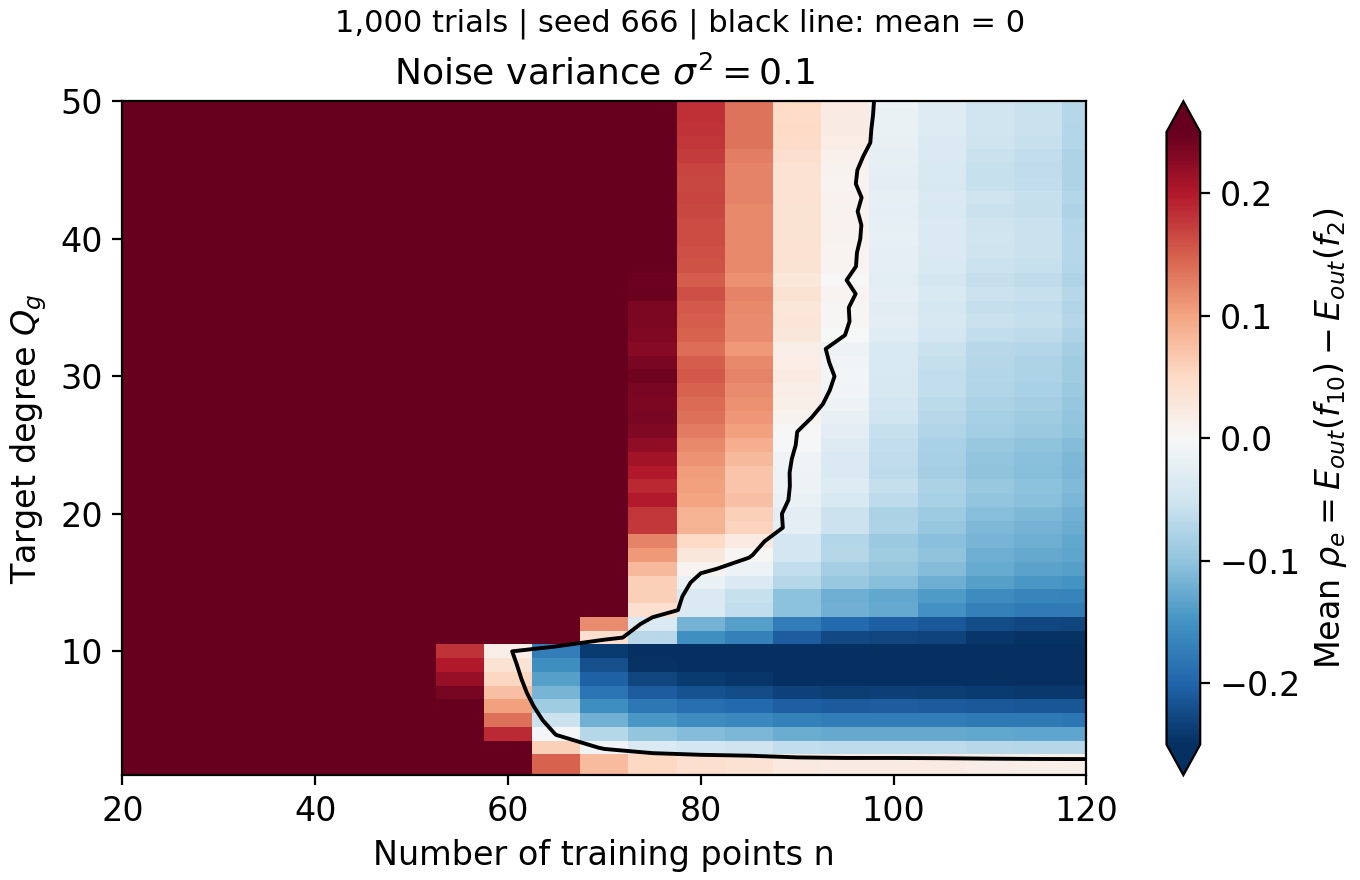
\includegraphics[width=.88\linewidth]{../results/run-20261027/p3/target_complexity.png}
\captionof{figure}{Target-complexity grid at fixed $\sigma^2=0.1$: horizontal axis $n=20,25,\ldots,120$, vertical axis $Q_g=1,\ldots,50$. Each cell averages all 1000 trials.}\label{fig:target}
\end{center}
\begin{center}
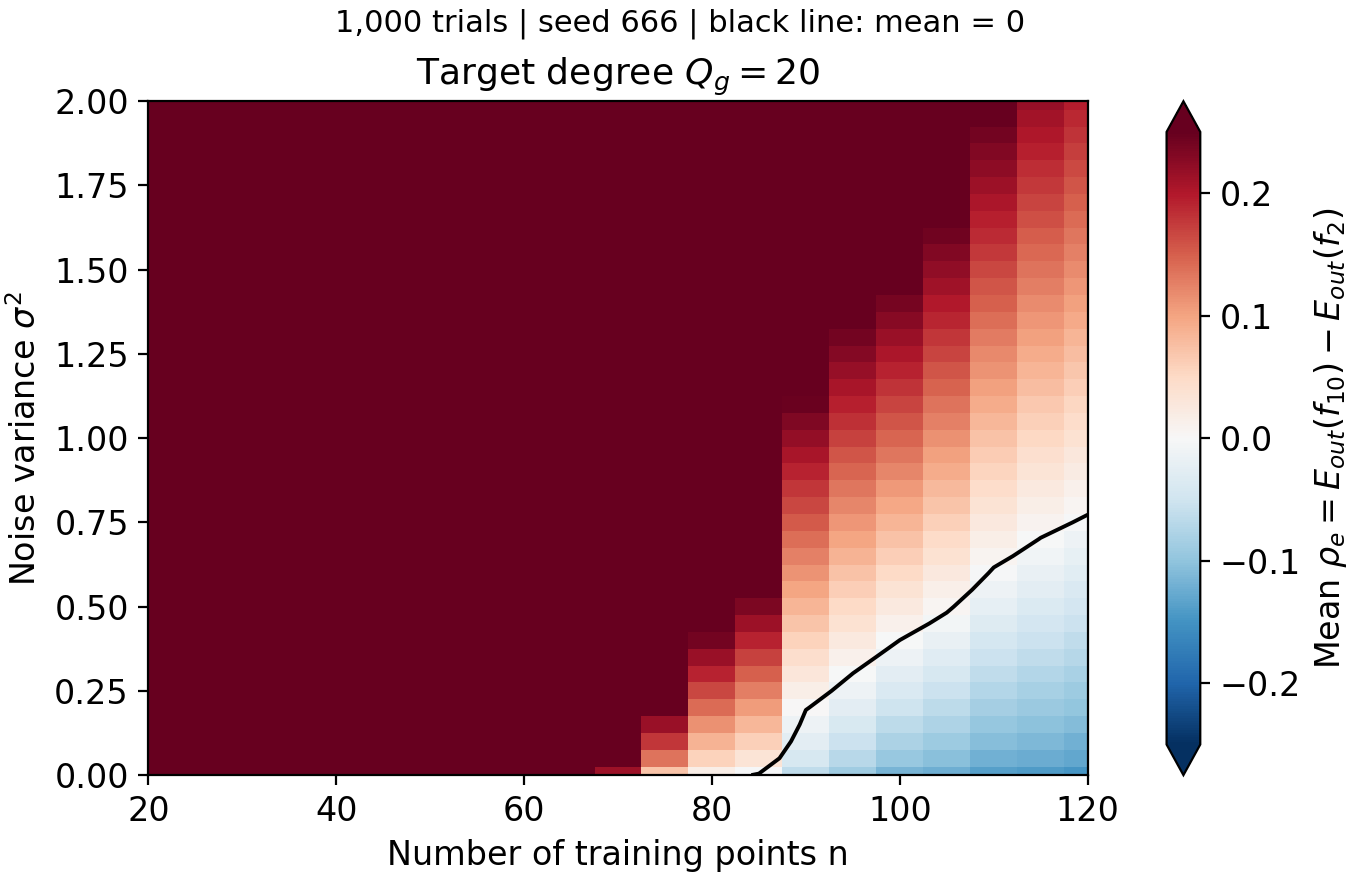
\includegraphics[width=.88\linewidth]{../results/run-20261027/p3/noise_variance.png}
\captionof{figure}{Noise-variance grid at fixed $Q_g=20$: the same horizontal sample counts and vertical axis $\sigma^2=0,0.05,\ldots,2$.}\label{fig:noise}
\end{center}

\clearpage
\section*{Problem 3(c): Interpretation}
\textbf{Colors and the zero contour.} Red means positive mean $\rho_e$: the degree-10 model has a larger clean-target error than the degree-2 model despite having no larger optimal training error. Blue means negative mean $\rho_e$, so degree 10 generalizes better in this particular comparison. White is near zero and the black contour marks the empirical zero-mean boundary. A negative value does not prove the degree-10 model cannot overfit relative to another model.

Colors saturate at $\pm0.25$ for visibility. The actual complexity-grid means range from $-0.296410$ to $1.032363\times10^6$, and noise-grid means from $-0.146917$ to $4.812316\times10^6$. These values were not clipped. Some finite-sample Legendre designs are poorly conditioned: the smallest recorded degree-10 design singular value is $1.304\times10^{-5}$. Large fitted coefficients can therefore amplify noise or model misspecification into large population errors, particularly where sample coverage is poor. All trials, including these extreme ones, contribute to the required arithmetic mean.

\textbf{Sample count.} More observations generally reduce the estimation instability of the flexible model in the observed grids and allow its approximation advantage to emerge. For example, at $Q_g=20$, $\sigma^2=0.1$, the mean error difference changes from about $968028.958439$ at $n=20$, to $11.581522$ at $n=40$, to $2.483317$ at $n=60$, and to $-0.119340$ at $n=120$. At $n=120$, the mean risks are $0.409165$ for degree 2 and $0.289825$ for degree 10. This is an observed tendency, not a theorem of monotonicity for each sample or every grid cell.

\textbf{Noise variance.} Noise can be fitted by the extra coefficients of $f_{10}$ and increase estimation variance. At $Q_g=20,n=120$, the means below move from a degree-10 advantage to a disadvantage as noise increases:
\begin{center}\small
\begin{tabular}{@{}rrrrr@{}}\toprule
$\sigma^2$ & $0$ & $0.1$ & $1$ & $2$\\\midrule
Mean $\rho_e$ & $-0.146917$ & $-0.119340$ & $0.037381$ & $0.196897$\\\bottomrule
\end{tabular}\end{center}
Finite paired Monte Carlo estimates need not be monotone at every cell. For example, at $n=40$ the zero-noise mean is $11.665551$ and the variance-$0.1$ mean is $11.581522$. Sample-specific cross terms can make such local comparisons nonmonotone; they are not grounds for discarding trials or changing the prescribed mean.

\textbf{Target complexity.} Increasing $Q_g$ is not always harmful. At $\sigma^2=0.1,n=120$, the mean $\rho_e$ is $0.014199$ for $Q_g=1$, $-0.071197$ for $Q_g=3$, $-0.296410$ for $Q_g=10$, and $-0.119340$ for $Q_g=20$. For targets of degree at most 2, both model classes contain the target and the extra coefficients mainly add noise-fitting variance. For intermediate degrees up to 10, the larger model can represent structure that the quadratic omits. Above degree 10, both models are misspecified; estimation error, omitted high-order components and the degree-dependent target normalization all matter. Consequently target degree alone does not determine the relative error.

\textbf{Can positive relative overfitting occur without observation noise?} Yes. The noise-grid mean at $\sigma^2=0,Q_g=20,n=20$ is $558740.582041>0$, whereas at $n=120$ it is $-0.146917$. With degree 20 the target is outside both fitted model classes, and fitting its values at a limited random set of inputs can induce a poor degree-10 approximation elsewhere, especially when the design is ill-conditioned. Observation noise is therefore not necessary. If the noiseless target were contained in the degree-10 class and the design had full column rank, an exact fit would instead recover it in exact arithmetic; this positive-error argument concerns the misspecified target case.

\textbf{Limits of the contour.} The displayed boundary is an empirical comparison of two models under this fixed random bank. The grids share random numbers, so adjacent cells are paired rather than independent. Within each cell there are 1000 independent trials, but rare large errors can strongly affect the mean: at $Q_g=20,\sigma^2=0.1,n=20$, its standard error is about $498426.190234$. The black line is not evidence of a universal sharp transition, nor a guarantee about an individual fitted model.


\section*{Execution and assistance disclosure}
The fixed experiments were actually executed on 27 October 2026 using Python 3.12.14, NumPy 2.2.6, SciPy 1.15.3, scikit-learn 1.7.2, Matplotlib 3.10.6 and threadpoolctl 3.7.0, on a CPU with numerical-library thread count limited to one by the original frameworks. The source functions, verification scripts, original runners/frameworks/tests and dependency list accompany this PDF. The small verification scripts require no datasets. Digits is included in scikit-learn; Dry Bean is downloaded from the fixed UCI URL and checked against the teacher's SHA-256. Data and raw trial archives are excluded from the submission as instructed.

Codex assisted with mathematical derivation, numerical implementation, test execution, experiment execution and English drafting. The dedicated AI page records the actual student--Codex verification question and numerical follow-up, translated from Chinese into English, with the source of the numerical evidence identified. Earlier coordinating-agent/coding-agent exchanges are also retained locally. Separate agents performed technical verification and final package review. The student remains responsible for understanding the submitted work and expressing mathematical derivations and explanations in their own words, as required by the assignment. This AI-assisted draft does not establish that a personal wording review has already occurred.

\end{document}
